\documentclass[10pt]{article}
\usepackage{geometry}
\usepackage{latexsym}
\usepackage{amsmath}
\usepackage{multirow}
\usepackage{url}
\usepackage[numbers]{natbib}
\usepackage{graphicx}
\usepackage{subcaption}
\newgeometry{margin=3.40cm}

\graphicspath{{../figures/}}

\title{{\large CS224W Project Milestone} \\
  What is karma? Quantifying online influence and credibility
}
\author{Thomas Dimson \\ {\tt tdimson@cs.stanford.edu}
  \and
  Milind Ganjoo \\ {\tt mganjoo@cs.stanford.edu}
}
\date{}

\begin{document}
\maketitle

%% TODO: Write and include abstract.
%% TODO: This is the expected format:
% We expect that you have completed 60% of the project
% Provide a complete picture of your project even if certain key parts have not yet been implemented/solved.
% Include the parts of your project which have been completed so far, such as:
% * Thorough introduction of your problem
% * Review of the relevant prior work
% * Description of the data collection process
% * Description of any initial findings or summary statistics from your dataset
% * Description of any mathematical background necessary for your problem
% * Formal description of any important algorithms used
% * Description of general difficulties with your problem which bear elaboration
% Make sure to at least outline the parts which have not yet been completed so that it is clear specifically what you plan to do for the final version.
% Recommended length 3-5 pages

\section{Introduction}
Many online communities explicitly publicize the concept of \textit{karma} or
\textit{reputation} for users, computed as a sum of positive votes by other members of
the community. These explicit measures are often seen as proxies for more
intangible notions such as \textit{influence} (the ability of a member to
persuade others) and \textit{credibility} (the trustworthiness of the user as an
member of the community). In this paper, we describe the range of network
characteristics, interactions, and temporal factors that affect the accumulation
of karma points. Using this, we build a model that predicts karma values.

Our topic is motivated by the class content discussing how users evaluate
each other in social graphs. We wish to determine whether network properties of the 
\textit{interaction graph} can explain karma metrics. Our subsequent model for 
could inform a general framework for quantifying influence and credibility
on other graphs (including those without \textit{users} as nodes).

\section{Data Collection}
For our report, we will be focusing on two communities: \textbf{Hacker News}
and the \textbf{StackExchange} family of websites. On Hacker News, users submit
technology-related stories as \textit{submissions} which other users
use as an anchor to threaded discussions. A user's \textit{karma} is computed
as a sum of up-votes to their stories and comments. The StackExchange family of 
websites are question-and-answer sites where a user will post a question and
solicit answers from the community. A user's \textit{reputation} is a weighted
sum based on the number of their questions and answers that are accepted, and
whether their comments and posts are voted as helpful by the community.

Gathering data for Hacker News came with many challenges: there is no published
dump of hacker news data, and no official API to help fetch. Fortunately, the creator
of ThriftDB has created HNSearch (\url{https://www.hnsearch.com/}) as a technology
demo for his database. In addition to a public website, there is an unofficial API
to support mechanical search queries. Although the API is limited to collecting 
only 100 recent items, we were able to circumvent this by constructing queries with limited
date ranges. Over the course of a week, we extracted JSON files for every comment,
submission and user on Hacker News by repeatedly querying the API. To our knowledge,
ours is the only complete dump of this data available on the internet.

%Milind can you talk about using SuperUser as a starting point, as well as discussing how
% you collected data. I think it is fine for this to be smaller than HN the dump is published

After collecting the raw data for both datasets, we created an SQLite database
with normalized columns for all the fields. We also created an interaction graph
by collecting $(\text{replier}, \text{parent poster})$ edges and then caching the graphs
on disk as a NetworkX structure. A summary of our datasets is available in 
Table~\ref{tab:graphstats}.

\section{Initial Findings}

\begin{figure}[h]
\centering
\begin{subfigure}{0.49\textwidth}
\centering
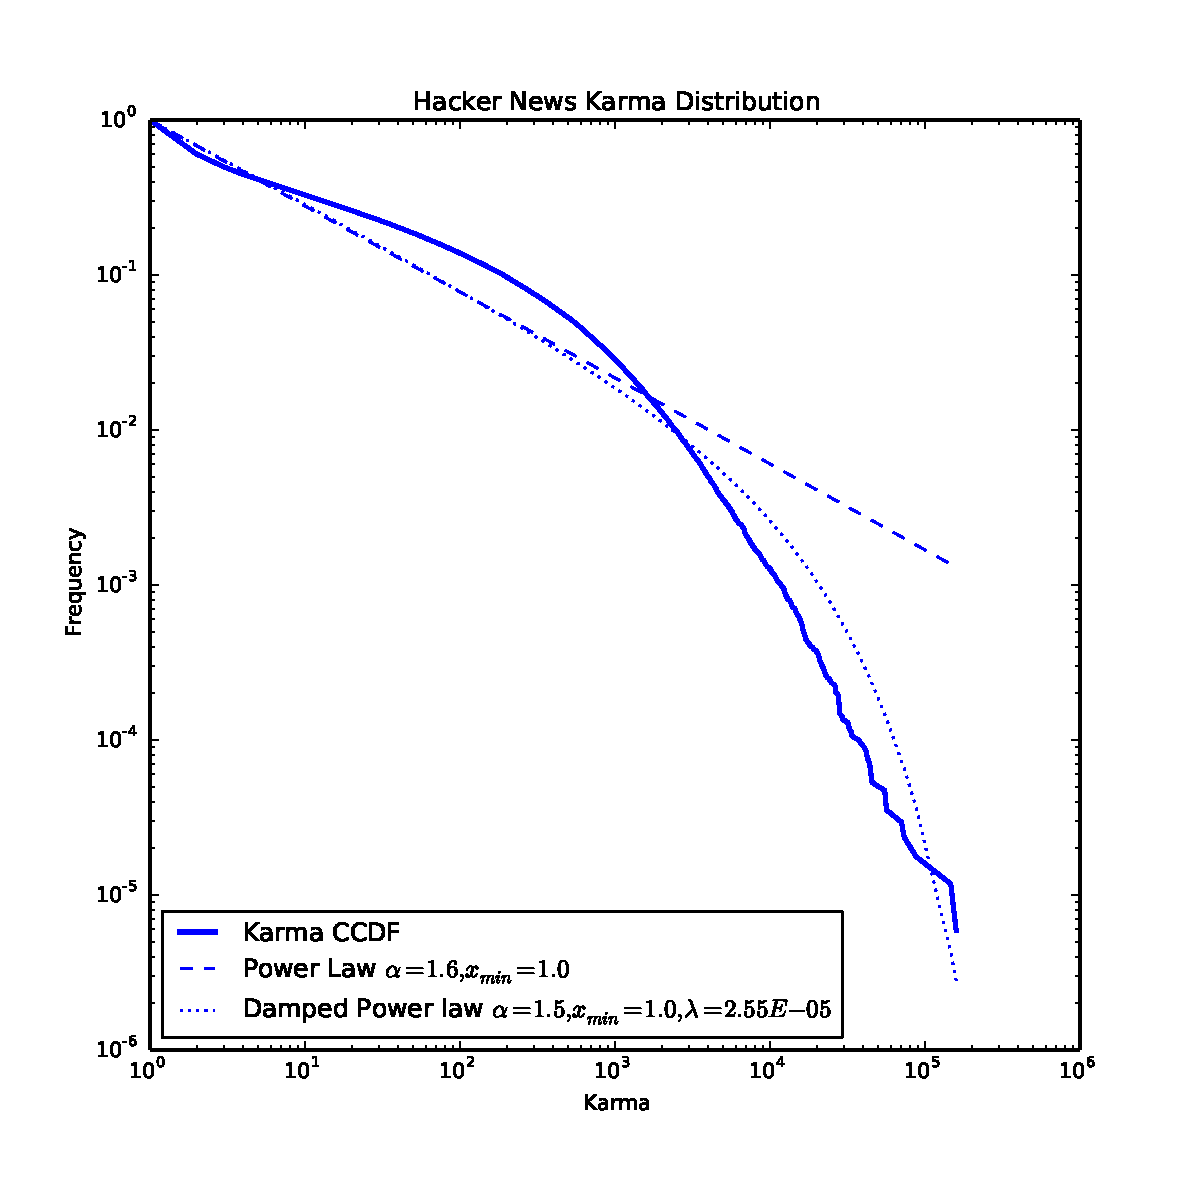
\includegraphics[width=\linewidth]{hn_karma_distribution}
\caption{Hacker News}
\label{fig:hnkarma}
\end{subfigure}%
\begin{subfigure}{0.49\textwidth}
\centering
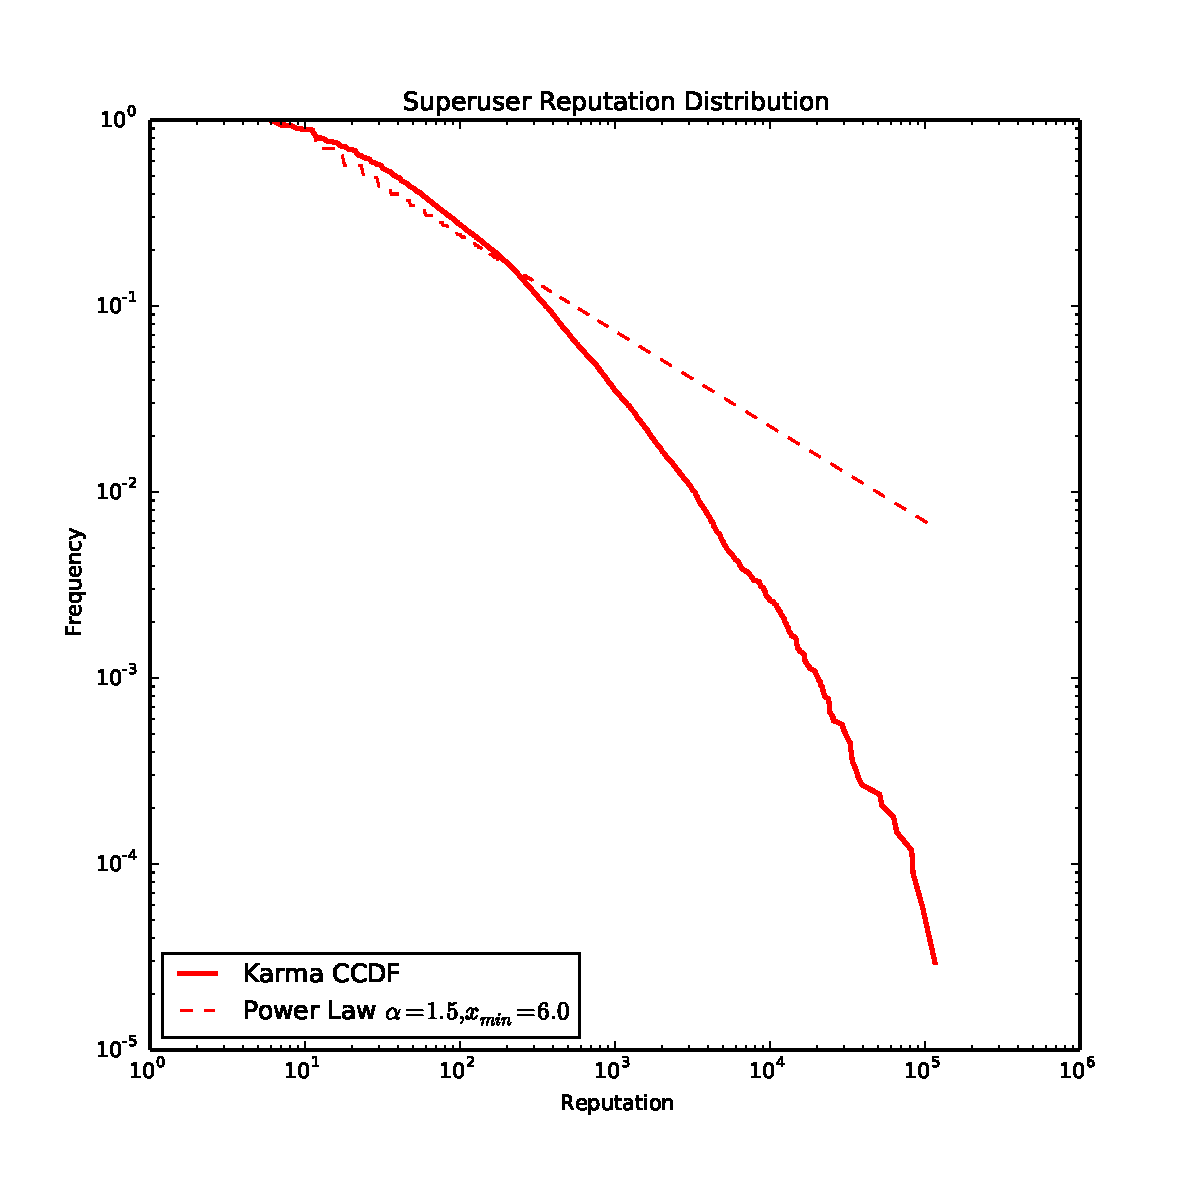
\includegraphics[width=\linewidth]{su_karma_distribution}
\caption{Super User}
\label{fig:sukarma}
\end{subfigure}
\caption{Karma distributions in our datasets with fitted power law distributions}
\label{fig:karma}
\end{figure}

\begin{table}[h]
\begin{center}
\begin{tabular}{| r | l l |}
\hline
& \textbf{Hacker News} & \textbf{Super User} \\
\hline
Users (Nodes) & 175091 & 190781 \\
Replies (Edges) & 2747966 & 266673 \\
Average Karma / Reputation & 131.8 & 83.1 \\
Largest SCC Fraction & 43\% & 3.8\% \\
Largest WCC Fraction & 63\% & 46\% \\
\hline
\end{tabular}
\end{center}
\caption{Graph statistics for our implied interaction graphs}
\label{tab:graphstats}
\end{table}

\begin{table}[h]
\begin{center}
\begin{tabular}{| r | l l |}
\hline
Model & \textbf{Hacker News RMSE} & \textbf{Super User RMSE} \\
\hline
Baseline &  & \\
Baseline+PageRank & & \\
Baseline+Weighted PageRank & & \\
\hline
\end{tabular}
\end{center}
\caption{Regression performance for our baseline and improved baseline models.}
\label{tab:regression}
\end{table}

\section{Next steps}
% Milind zone

\section{Conclusion}
% Milind zone


\section{Literature review}
\subsection{Everyone's an influencer: quantifying influence on Twitter \citep{bakshy2011everyone}}

\citet{bakshy2011everyone} define \textit{influence} as the ability to generate
cascades containing URLs on Twitter. Technically, they begin by examining the
first tweet (seed) containing the URL and then measure how the URL propagates
through the seed user's follower tree. To measure their success, they train a
model that attempts to predict cascades based on attributes of the user (e.g.,
number of followers or the number of tweets) and their past ability to generate
cascades.  Unsurprisingly, the past ability to predict cascades was the best
predictor of future performance.

A big take-away from this paper is that local features -- those from a user's
immediate followers -- are better indications of influence than global ones
(wider properties of the graph). The authors also use Mechanical Turk to
categorize tweeted URs in an attempt to see if cascades are affected by the
\textit{content} of the tweets. They admit that this categorization did not help
in their prediction task. 

\subsubsection{Analysis of the Reputation System and User Contributions on a
  Question Answering Website: StackOverflow
  \citep{movshovitzanalysis}}

In this very recent paper, \citet{movshovitzanalysis} consider the reputation
scheme on StackOverflow (based on upvotes and accepted answers). They analyze 9
million questions and answers posted by 1.2 million users since the site's
inception and attempt to identify expert users based on their contribution
patterns.

One striking direction pursued by the paper is their use of PageRank on
interaction graphs implied by the questioner and answerer (stratified into three
different graphs based on whether the answer was upvoted, accepted, or neither).
They attempted to find important nodes (users) through this approach. However,
they observed that reputation scores are not as correlated with PageRank values
as they had originally thought -- many users with high reputation had
relatively low PageRank.

In addition to PageRank, the paper attempts to find anomalous users by running
SVD on the interaction graphs This yielded a few anomalous questioner and
answerer users, who gained extremely large reputations and had highly focussed
ego networks, mainly through only one type of contribution (i.e.\ either a
question or an answer). We note the illustratation of the non-overlapping ways
reputation can be built, and informs an approach to filter out anomalies.

Finally, this paper builds a classification model to predict ``expert users'',
defined as users with reputation scores of more than 2400. They build a
binary classification model based on user features such as number of answers,
questions, accepted answers, upvoted answers and comments, and question-answer
ratios. Using a random forest classifier, they obtain an Area
under the Curve of 81\% -- which they claim is higher than previous attempts.


\subsubsection{Measuring User Influence in Twitter: The Million Follower Fallacy
  \citep{cha2010measuring}}

Like \cite{bakshy2011everyone}, \citet{cha2010measuring} study a more practical
implication of influence: the ability of a user to spread information to a
large network of nodes. The paper compares three measures of influence of
Twitter users: in-degree, number of retweets earned, and number of mentions.
They use the \textit{rank correlation coefficient} to compare measures of
influence:

\begin{equation}
  \rho = 1 - \frac{6\sum{(x_i - y_i)^2}}{N^3 - N}
\end{equation}

where $x_i$ and $y_i$ are the ranks of users based on two different influence
measures. Using this, they found that the users with high number of mentions
also get retweeted often, i.e.\ there is high correlation between retweet and
mention influence. However, the in-degree (number of followers) was not
correlated to other measures, indicating that merely having a large number of
followers says nothing about the ability to practically engage with one's
audience.

Another conclusion of this paper is that the users with highest mention
influence were usually famous people like celebrities (indicating the
\emph{name} value of mention influence), while high retweet influence was
associated with content aggregators like news accounts (indicating the
\emph{content} value of retweet influence).

The paper also emphasizes the topic-specificity of influence -- they challenge
the notion that there is a common set of ``influentials'' who have
broad-reaching impact on online communities. Instead, they demonstrate that for
many topics, such as political events, there are special interest groups like
bloggers and politicians that see higher retweet and mention scores than the
generally popular Twitter users.

The final contribution of this paper is a temporal analysis of influence. In
particular, they study how influence wanes over time (measured by changing retweet
and mention probabilities $P$) when not maintained through regular engagement
with the community. Additionally, they track influence gains by select users
to explain the often meteoric rise in influence of topical posters during major
events.

\subsection{Critique} 
Both \citet{bakshy2011everyone} and
\citet{cha2010measuring} consider \textit{influence} in the Twitter graph, as
defined by the ability to generate cascades. One of the broader issues is that
influence is a conceptual quality instead of something directly measureable.
Unlike karma, there isn't a notion of a \textit{gold standard} from which
cascades can be measured.  We feel these papers could be greatly strengthened
by linking their analysis to an observable quantity instead of an abstract
concept.

The role of content isn't particularly well-explored in either of the Twitter papers.
Specifically, we take issue with the \citet{bakshy2011everyone}: they analyze
the role of content in cascades by hand-classifying the tweets by Mechanical Turk.
The details of this process are somewhat sparse in the paper and the human
dependency makes their dataset limited in size and scope. We believe a better
approach would be to cluster tweets/URLs by their words, for example by
a topic modelling algorithm such as Latent Dirichlet Allocation (LDA)
\citep{blei2003latent}. Although the clusters would not be perfect, the assignments
would give an objective category by which to compare the role of cascades.

A similar lack of content focus can be seen in \citet{cha2010measuring}. Their
topic-specific analysis of tweets relied on specific keywords associated with
three prominent events. We feel the use of automated topic modelling would help
yield a more extensive and diverse dataset.

Temporal analysis of influence is an area we wish to study but
the analysis by \citet{cha2010measuring} was not comprehensive
They tracked the change in influence only for 100 top users, and
their explanation for trends, by their own admission, was mostly 
based on manual appraisal of tweet content for users that became popular.
We could consider performing a more rigorous graph-based analysis when looking at temporal
trends. We are more optimistic since our data
could contain temporal information attached to each user-user interaction,
and thus allows us to look at the history of the interaction graph. In contrast, this
re-tweet and mentino data is often incomplete for Twitter.

\citet{movshovitzanalysis} analyze a different dataset (StackOverflow
reputation) in a concrete, mathematical fashion.  One of the shortcomings of
this paper is that it notes discrepancies betwen reputation scores and PageRank
(namely that the two don't often correlate positively for many users), but does
not attempt to explain them. Specifically, we could consider performing
topic-sensitive PageRank and LDA (described in Section~\ref{sec:models}) to see
if stronger correlation occurs in the context of topics.  Additionally, we would
like to perform other forms of stratification, such as setting thresholds on
interaction length, to calculate PageRank framed within long and potentially
insightful interactions.

Instead of identifying expert users through a classification task, we could
consider a generalizable model to predict karma scores directly. The model's
parameters may vary depending on the nature of our data sources. Still, their
work seems like a natural and high-performing baseline for our evaluations. 

\subsection{Brainstorming and Future Directions}

Two of our papers address the concept of influence in the Twitter graph, where
it is not directly observable. We are intrigued by their definition of influence
as the ability to create cascades of networks, but think that it might be better
validated on a graph that has an explicit notion of \textit{influence}.

\citet{movshovitzanalysis} has a more quantitative analysis of reputation on
StackOverflow.  Although they don't address cascades directly, we are fascinated 
by the structured approach they take to their analysis and believe it could apply
to our own techniques.  StackOverflow has a particularly complicated
notion of reputation, which is not simply a linear combination of up-votes to
pieces of content. Analyzing a similar quantity on more direct graphs (e.g.,
karma on Slashdot) might make for a more successful model.

Furthermore, the paper has a concrete evaluation metric: the ability to predict
``influentials'' (high karma individuals). We could try to pursue a similar
direction, but it makes more sense to us as a regression problem (predicting
karma) than a classification (predicting large karma).

All the literature we read contained a large descriptive section. This provided
a very natural progression between ideas and models. In our paper, we could
start by first looking at factors correlated with karma and then use this
analysis as a base for our model. Additionally we could also look at social
interactions to see, for example, if high karma users always reply to other high
karma users.

The temporal analysis in \citet{cha2010measuring}, while rudimentary, does
underscore the changing nature of influence. On the other hand, karma scores on
most websites are static, and often may not present the latest and most
realistic picture of the influence and credibility of the user. 
When analyzing karma values, we would need to sift out users with high values
who gained points over short and irregular bursts of activity, compare them
against users who have been long-standing members of the community, and look for
explanatory trends and differences.

Finally, we consider focusing some of our analysis exclusively on the set of
high karma users. Our hope is that some intangible aspects of karma come to
light, such as the nature, tone and quality of interaction among top users. We
could also test the veracity of the anecdotal ``power struggle'' between top
members of online communities.

\section{Project Proposal} \subsection{Problem Definition}
% What is the problem we are solving
Our term will be spent creating a mathematical model of user karma that is
validated by its ability to predict karma values for individual users. We want
to answer the question: is karma simply the sum of positive votes for a given
user, or is it also predicted by wider properties of the social graph?
Furthermore, is our model of karma specific to a single website or does it apply
more broadly across different datasets?  Finally, on sites that lack an explicit
model of karma (e.g. Wikipedia), does our model identify high-scoring nodes that
match our intuition?

\subsection{Data Sources}
% What data sources are we using and how will we collect it
We will be using multiple data sources in our project. As part of a past
project in Natural Language Understanding (CS224U), we crawled a large dataset
of conversation trees on the popular ``Hacker News''
(\url{https://news.ycombinator.com/}) website, containing nearly 100,000
messages. On the site, users submit stories (URLs) which are up-voted by other
users. Each story is accompanied by comments, in the form of a threaded
conversation tree, which are also up-voted and down-voted by different users.
Each user on the site has a visible karma score, which is the sum of all
upvotes and downvotes that their comments and stories have received.  We
anticipate building a comment \textit{graph} of users where directed edges
represent the source replying to the target in a conversation.

As a secondary datasource, we would also like to analyze StackOverflow
(\url{http://stackoverflow.com/}). Here, a poster creates a programming-related
question and solicits answers from the community. When satisfied, the poster
marks their question as ``solved''. Other members of the community can up-vote
or down-vote both questions and answers. Each user on the site has a
``reputation'', which is a weighted combination of up-votes, down-votes and
other factors such as question creation and closed answers. Fortunately,
StackOverflow makes all their data available online through their StackExchange
data explorer (\url{http://data.stackexchange.com/}) and we will not have to
perform any crawling to get access.

\subsection{Anticipated Work}
% What work do you plan to do the project?
Development of our project will begin with a \textit{descriptive} component. The
obvious first step is to take karma and visualize it: does it follow a power
law?  Is the power law different depending on the data source we analyze? Having
determined what karma looks like, we can start to see how it correlated to wider
properties of the graph. For example, we could look at how the clustering
coefficient varies with karma of the user.

After making sense of the data we are dealing with, we anticipate moving towards
our \textit{predictive} component. Guided by our earlier findings we will try to
create a model that is able to perform blind-prediction on karma. It seems
plausible that some of our early metrics could play the role of
\textit{features} in this system.

\subsection{Models and Algorithms}
\label{sec:models}
% Which algorithms/techniques/models you plan to use/develop? Be as specific as you can!
The final model we produce will likely be a regression model fit on top of
features that we identify in the descriptive phase of our project. Ideally, we
would be able to take the model we create for our \textit{Hacker News} dataset
and achieve similar results on our \textit{StackOverflow} dataset with a small tweak
in our parameters. If a regression model proves to be impossible due to the wide
variance in karma scores, we could also evaluate our success on a classification
task that attempts to divide users into high-karma (important contributors) and
low-karma users (unimportant contributors) by picking a fixed threshold of karma
scores.

We are particularly interested in exploring the role of \textit{content} in
karma. Specifically, we want to know if there are different karma distributions
for users depending on the topics that they normally discuss. We could
investigate this by computing topic-distributions for users through Latent
Dirichlet Allocation (LDA). We could then look at probability-weighted karma
distributions in each topic, and see if there is a wide variance between topics.
Depending on the answer, we could consider creating different models for each
topic. Furthermore, we could try to evaluate topic-coherence in the
neighborhoods around each node (do people talk to each other about the same
things?).

On the surface, PageRank feels like a natural fit for our task because it
generally corresponds to the \textit{authority} or \textit{influence} of nodes
in our graph. A component of our analysis will be to plot karma against PageRank
scores to see how predictive we can be.  Going deeper, we could combine our
LDA-topic analysis with PageRank by performing Topic-Sensitive PageRank
\citep{haveliwala2002topic} on our nodes and seeing if graph authority is more
predictive of karma within certain topics. This hypothesis was validated in
predicting following relationships on the Twitter graph in
\citet{weng2010twitterrank}

\subsection{Evaluation}
% Who will you evaluate your method? How will you test it? How will you measure
% success?
Since karma is directly observable, we will test our model in a
blind-prediction task. Concretely, we will run our model on a dataset without
looking at the ``gold'' karma scores and then evaluate our prediction quality
based on the average residual between the gold score and our predicted score.

We will frame the quality of our results by evaluating them against a simple
baseline: least squares regression using the number of replies by the poster and
length of time the poster has been a member of the site. According
to~\citet{movshovitzanalysis}, these were two strong indicators of reputation on
StackOverflow. 

\subsection{Submission}

Our final submission will address what the concept of \textit{karma} means on
different websites on the web. Our paper will begin by analyzing the
distribution of karma and proceed to correlate karma scores with basic graph
measurements (e.g., clustering coefficients). Guided by this analysis, we intend
to build up a mathematical model of karma and create a regression model for
prediction. This model will be evaluated in a blind-prediction task and measured
against a simple baseline. Time permitting, we will also apply our
model to a dataset where karma is latent and see how well it stacks up
against our intuition.

\bibliographystyle{abbrvnat}
\bibliography{milestone}

\end{document}
